\documentclass{article}
\usepackage[T1]{fontenc}
\usepackage{lmodern}
\usepackage{graphicx}
\usepackage{amsmath,amssymb}
\usepackage[a4paper,margin=2cm]{geometry}
\usepackage[absolute,overlay]{textpos}
\setlength{\TPHorizModule}{1mm}
\setlength{\TPVertModule}{1mm}
\usepackage[indonesian]{babel}
\usepackage{hyperref}
\setlength{\emergencystretch}{2em}
% unit: Halaman 9

\begin{document}

% === Halaman 9 (llm) ===

\section*{Mode Operasi \textit{Cipher} Blok}

\vspace{130.68mm}

\begin{itemize}
    \item Mode operasi: berkaitan dengan cara blok pesan dioperasikan sebelum dienkripsi/dekripsi oleh fungsi E dan D.
    \item Ada 5 mode operasi \textit{cipher} blok:
    \begin{enumerate}
        \item \textit{Electronic Code Book} (ECB)
        \item \textit{Cipher Block Chaining} (CBC)
        \item \textit{Cipher Feedback} (CFB)
        \item \textit{Output Feedback} (OFB)
        \item \textit{Counter Mode}
    \end{enumerate}
\end{itemize}

\vspace{10mm}

% deskripsi: Diagram blok proses enkripsi dan dekripsi menggunakan fungsi E dan D dengan kunci K, menunjukkan transformasi dari blok plaintext P menjadi blok ciphertexts C dan sebaliknya.
% bbox normalisasi: [0.5200, 0.4000, 0.9600, 0.8400]
\begin{textblock*}{92.40mm}(109.20mm,118.80mm)
\noindent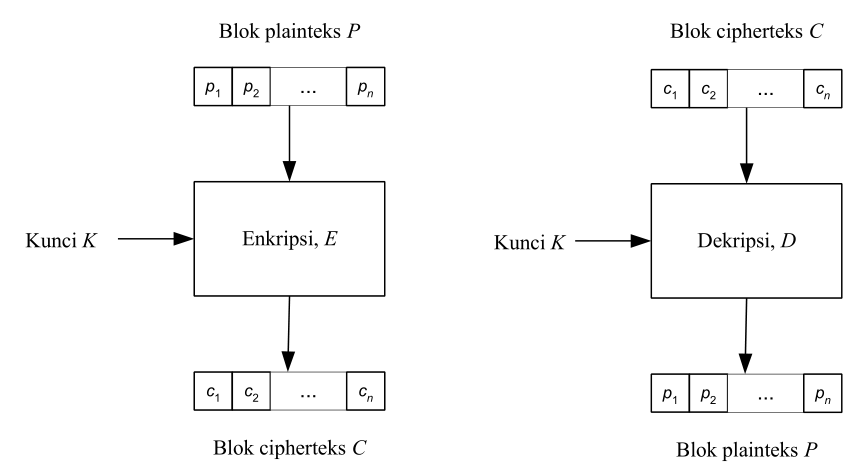
\includegraphics[width=92.40mm,height=130.68mm]{../../images/llm/page_009_img_01.png}%
\end{textblock*}

\end{document}
